\chapter{Estado da arte}

Estado da arte revisto; trabalho relacionado.

\section{Citações}
Exemplo de uma citação: \cite{GRM97}, cf. esta entrada em \texttt{dissertation.bib}.
Outra forma de citar \citep{KeR88}.

\section{Expressões matemáticas}
A equivalência massa-energia é descrita pela famosa equação
\begin{equation}
E=mc^2
\end{equation}
descoberta em 1905 por Albert Einstein.
Em unidades naturais ($c = 1$), a fórmula expressa a identidade
\[
E=m
\]

\section{Notas de rodapé}
Este é um exemplo de uma nota de rodapé\footnote{The quick brown fox jumps over the lazy dog.}.

\section{Acrónimos e Glossário}
\newacronym{gcd}{MDC}{
Máximo Divisor Comum}
\newacronym{lcm}{MMC}{Mínimo múltiplo comum}
\newglossaryentry{maths}
{
    name=matemática,
    description={Matemática é o que os matemáticos fazem}
}
\newglossaryentry{latex}
{
    name=latex,
    description={É uma linguagem especialmente adequada para
documentos científicos}
}
\newglossaryentry{formula}
{
    name=fórmula,
    description={Expressão matemática}
}

Dado um conjunto de números, existem métodos elementares para calcular
seu \acrlong{gcd}, que é abreviado como \acrshort{gcd}. Este processo
é semelhante ao usado para o \acrfull{lcm}.

O \Gls{latex} é especialmente adequado
para documentos que incluam \gls{maths}. \Glspl{formula} são corretamente e facilmente renderizados a partir do momento que nos habituamos aos comandos.

\section{Índice}

Neste exemplo, várias palavras-chave\index{palavras-chave} importantes serão usadas pelo que merecem aparecer no Índice\index{Índice}.

Os termos no índice também podem ser aninhados \index{Índice!aninhados}.

Cf. o ficheiro \texttt{dissertation.bib} para ver algumas definições como \uminho{UMinho}.

%%%%%%%%%%%%%%%%%%%%%%%%%%%%%%

\chapter{Estado da arte}

%Estado da arte revisto; trabalho relacionado.
A gestão de consentimento é um dos principais desafios no tratamento de dados pessoais, especialmente face ao crescimento exponencial da digitalização e às regulamentações como o \acrshort{rgpd}. As \acrshort{cmp}s surgem como uma solução prática para facilitar a recolha e a gestão do consentimento do utilizador, assegurando a conformidade com estas legislações. No entanto, enquanto as \acrshort{cmp}s oferecem mecanismos para gerir o consentimento, existem limitações em termos de transparência e auditabilidade.


\section{\acrfull{cmp}}

As \acrfull{cmp} desempenham um papel essencial ao fornecer aos \textit{titulares dos dados} uma forma clara e explícita de consentir com o tratamento dos seus dados pessoais. Estas plataformas surgiram como resposta à crescente necessidade de garantir que os direitos dos Titulares dos Dados sejam respeitados no contexto da recolha e tratamento dos seus dados, especialmente face às exigências do \acrshort{rgpd}. A principal função das \acrshort{cmp}s é proporcionar uma solução eficaz e transparente para a obtenção, armazenamento e gestão do consentimento dos Titulares dos Dados, garantindo que as organizações cumpram as obrigações legais impostas pelas regulamentações de privacidade. Estas plataformas permitem que os Titulares dos Dados tenham controlo sobre o uso dos seus dados pessoais e são devidamente informados sobre as práticas de tratamento destes mesmos.

Entre as soluções mais populares encontrou-se plataformas como \textbf{Osano}, \textbf{Cookiebot}, \textbf{Tarteaucitron.js}, \textbf{Klaro.js} e \textbf{Consent Manager}. Cada uma destas plataformas oferece funcionalidades específicas, mas todas têm em comum o foco na conformidade com as regulamentações de privacidade, como o \acrshort{rgpd}.

\begin{itemize}
    \item \textbf{Osano}: Oferece uma interface intuitiva de personalização e um sistema eficiente de gestão de preferências \cite{osano}. Inclui recursos avançados como armazenamento local de preferências e bloqueio automático de rastreamento não autorizado. Contudo, por ser uma solução proprietária, apresenta limitações na verificação do processamento de dados entre o navegador e o servidor.

    \item \textbf{Cookiebot}: Fornece uma solução robusta que analisa automaticamente até 10.000 páginas por domínio \cite{Cookiebot2024}. Implementa um sistema inteligente para detetar mudanças nos \textit{cookies} e rastreadores do site. A principal limitação 
    está na sua natureza fechada do código, que dificulta verificações independentes do funcionamento interno.

    \item \textbf{Tarteaucitron.js \& Klaro.js}: São soluções de código aberto que se destacam pela flexibilidade \cite{tarteaucitron}. O Tarteaucitron.js permite extensões personalizadas e um carregamento otimizado de \textit{scripts}, enquanto o Klaro.js oferece um sistema flexível de armazenamento de preferências e suporte a múltiplos idiomas. Ambos permitem personalização completa do controlo de \textit{cookies}.

    \item \textbf{Consent Manager}: Utiliza uma estrutura moderna que permite sincronização instantânea das preferências do utilizador entre diferentes \textit{tabs} do navegador \cite{ConsentManager2024}. Embora ofereça recursos avançados de gestão, devido à sua natureza fechada, limita a possibilidade de auditorias independentes.

    \item \textbf{CookieChimp}: Diferencia-se pela facilidade de integração com outros sistemas e pela gestão eficiente de consentimento \cite{CookieChimp2024}. Disponibiliza uma \acrshort{api} RESTful bem documentada que permite integração simples com sistemas externos.
\end{itemize}


Apesar dessas soluções estarem bem posicionadas para garantir a conformidade legal, um problema recorrente nas \acrshort{cmp}s existentes é a falta de visibilidade sobre os dados transmitidos. Os utilizadores podem não saber exatamente o que acontece com as suas informações depois de fornecerem o consentimento. Não há uma forma clara e acessível para verificar se as escolhas feitas são efetivamente respeitadas, o que levanta questões sobre a transparência e a auditoria.

\subsection{Fluxo de Implementação de uma \acrshort{cmp}}

Para ilustrar a necessidade destas plataformas, considere-se o seguinte cenário: um desenvolvedor cria um site e precisa garantir que o tratamento de dados dos visitantes esteja em conformidade com o \acrshort{rgpd}.

O fluxo típico para garantir essa conformidade pode ser representado no diagrama de atividades da Figura~\ref{fig:diagrama-cmp}, apresentada em seguida.

\begin{figure}
\begin{center}
    \begin{tikzpicture}[node distance=2cm]

        \node (A) [inicio] {Desenvolvedor cria site};
        \node (B) [processo, below of=A] {Integra \acrshort{cmp} (ex: CookieChimp)};
        \node (C) [processo, below of=B] {Configura \acrshort{cmp} e adiciona JavaScript};
        \node (D) [inicio, below of=C] {Utilizador acessa site};
        \node (E) [processo, below of=D] {\acrshort{cmp} exibe banner de consentimento};
        \node (F) [decisao, below of=E, yshift=-1cm] {Utilizador decide};

        \node (G1) [processo, right of=F, xshift=4cm] {Aceita todos os \textit{cookies}};
        \node (G2) [processo, below of=F, yshift=-1cm] {Recusa \textit{cookies} não essenciais};
        \node (G3) [processo, left of=F, xshift=-4cm] {Personaliza preferências};

        \node (H) [processo, below of=G2] {\acrshort{cmp} armazena preferências};
        \node (J) [processo, below of=H] {Decisão registada (\textit{Dashboard} CookieChimp)};
        \node (K) [processo, below of=J] {Utilizador pode alterar preferências};

        % Conexões
        \draw [seta] (A) -- (B);
        \draw [seta] (B) -- (C);
        \draw [seta] (C) -- (D);
        \draw [seta] (D) -- (E);
        \draw [seta] (E) -- (F);
        \draw [seta] (F) -- (G1) node[midway, above] {Aceita tudo};
        \draw [seta] (F) -- (G2) node[midway, right] {Recusa};
        \draw [seta] (F) -- (G3) node[midway, above] {Personaliza};
        \draw [seta] (G1.south) |- (H);
        \draw [seta] (G2) -- (H);
        \draw [seta] (G3.south) |- (H);
        \draw [seta] (H) -- (J);
        \draw [seta] (J) -- (K) node[midway, right] {Se desejar};
    \end{tikzpicture}
\end{center}
    \caption{Fluxo de implementação de uma \acrshort{cmp} num site.}
    \label{fig:diagrama-cmp}
\end{figure}

\newpage

O processo pode ser descrito da seguinte forma:

\begin{enumerate}
    \item O desenvolvedor cria um site.
    \item Para cumprir o \acrshort{rgpd}, decide integrar uma \acrshort{cmp}, como o \textbf{CookieChimp}.
    \item Escolhe uma plataforma e configura a ferramenta escolhida, adicionando o seu código JavaScript ao site.
    \item Quando um utilizador acessa o site, o \textit{plugin} da \acrshort{cmp} exibe um \textit{banner} (fig. \ref{fig:banner}) solicitando consentimento.
    \item O utilizador pode:
          \begin{itemize}
              \item Aceitar todos os \textit{cookies} e tecnologias de rastreamento.
              \item Recusar todos os \textit{cookies} não essenciais.
              \item Personalizar as suas preferências, selecionando categorias específicas (ex: marketing, estatísticas, essenciais).
          \end{itemize}
    \item A \acrshort{cmp} armazena as preferências do utilizador e bloqueia os \textit{cookies} de terceiros até que o consentimento seja dado.
    \item A decisão do utilizador é registada e pode ser consultado pelo criador do site, via dashboard do \textbf{CookieChimp} como pode ser visto na figura \ref{fig:dashboard-visualizacao}.
    \begin{figure}[h]
    \begin{center}
	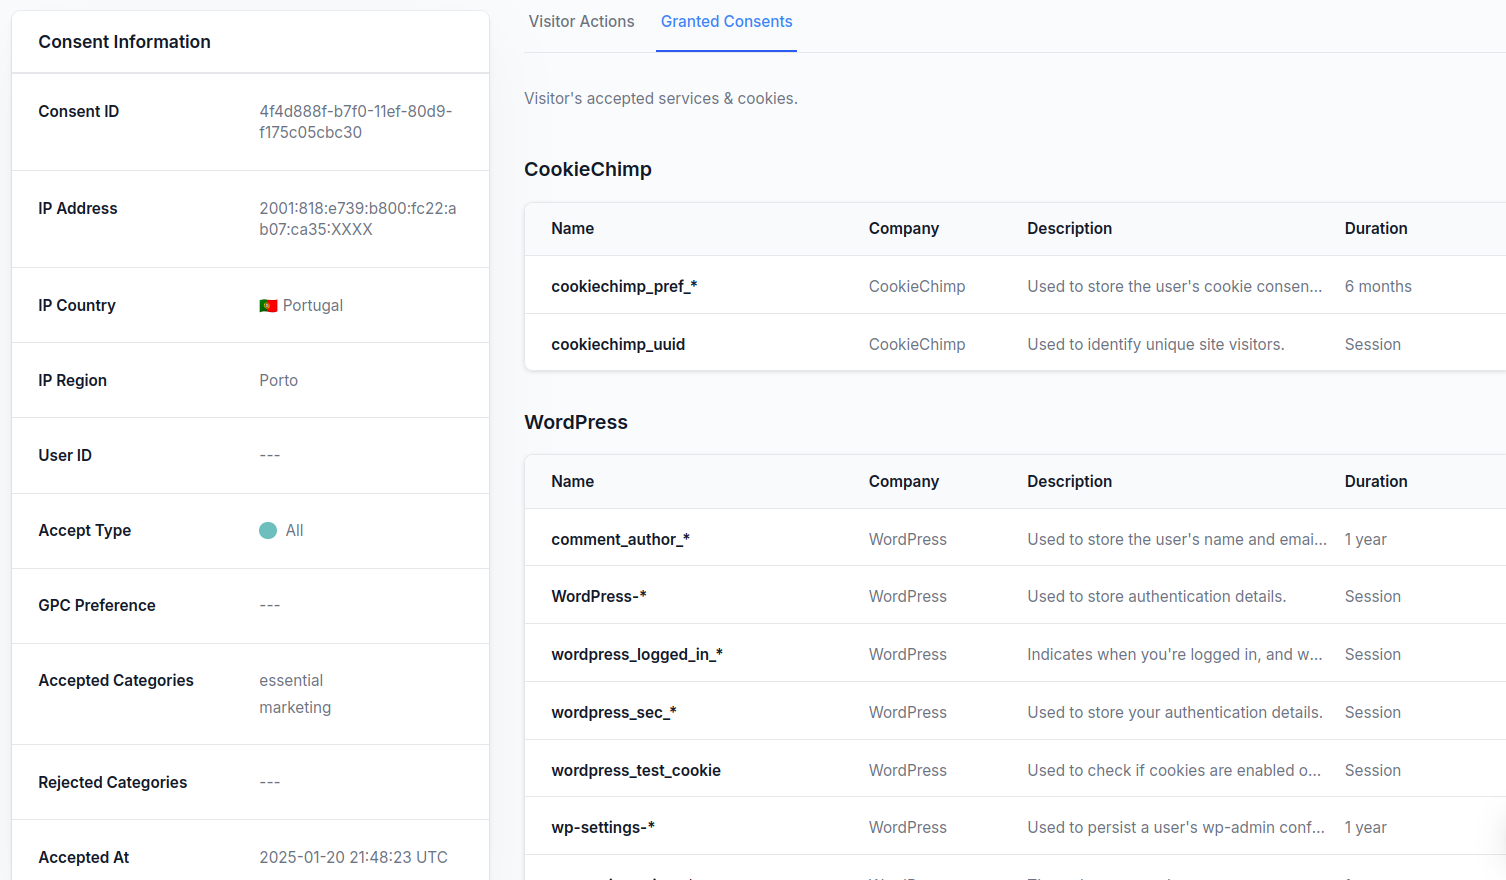
\includegraphics[width=0.8\textwidth]{images/consent.png}
    \end{center}
    \caption{Exemplo de visualização do consentimento na \textit{dashboard} do CookieChimp.}
    \label{fig:dashboard-visualizacao}
    \end{figure}
    \newpage
    \item Se o utilizador desejar alterar as preferências, pode fazê-lo através de um botão de configuração acessível no site.
\end{enumerate}

Desta forma, as \acrshort{cmp}s garantem transparência e conformidade com as regulamentações de privacidade, permitindo que os utilizadores tenham maior controlo sobre os seus dados pessoais.

\begin{figure}[h]
\begin{center}
	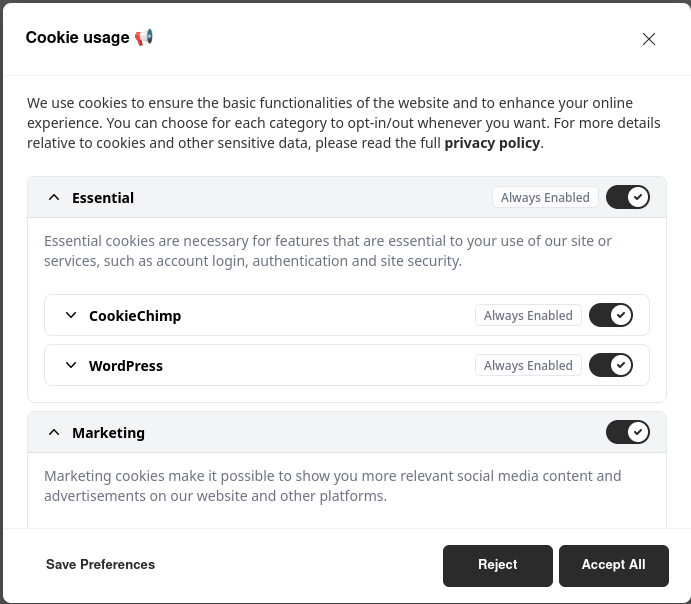
\includegraphics[width=0.8\textwidth]{images/banner.png}
\end{center}
\caption{Exemplo de banner de consentimento exibido ao utilizador.}
\label{fig:banner}
\end{figure}

\newpage

% \section{Limitações das CMPs Existentes}

% As CMPs tradicionais, embora eficientes na recolha e gestão do consentimento, têm algumas limitações notáveis, nomeadamente:

% \begin{itemize}
%     \item \textbf{Falta de transparência}: Muitas das CMPs atuais não permitem uma visão clara sobre como os dados dos utilizadores são processados ou armazenados após o consentimento. Em muitos casos, os utilizadores não sabem se o consentimento foi transmitido corretamente ao servidor ou se as suas escolhas estão a ser respeitadas.

%     \item \textbf{Ausência de auditoria eficaz}: A capacidade de auditar o processo de consentimento em tempo real é limitada. As CMPs existentes geralmente não oferecem mecanismos robustos para garantir que os dados estão a ser recolhidos e processados de forma conforme às escolhas do utilizador.

%     \item \textbf{Soluções fechadas}: Muitas das principais CMPs do mercado são soluções fechadas, o que dificulta a transparência sobre os seus processos internos. O código-fonte não é acessível ao público, o que impede que pesquisadores ou outras partes interessadas possam verificar a conformidade com as regulamentações de privacidade.
% \end{itemize}

\section{Limitações das \acrshort{cmp}s Existentes}

As \acrshort{cmp}s desempenham um papel crucial ao fornecer aos utilizadores uma forma de consentir explicitamente com o uso dos seus dados pessoais. Entre as soluções mais populares, destacam-se \textbf{Osano}, \textbf{Cookiebot}, \textbf{Tarteaucitron.js}, \textbf{Klaro.js}, \textbf{Consent Manager} e \textbf{CookieChimp}. Cada uma destas plataformas oferece funcionalidades específicas e foca-se na conformidade com regulamentações de privacidade, como o \acrshort{rgpd}. No entanto, apesar da sua importância, essas plataformas apresentam várias limitações que comprometem a transparência, a auditabilidade e a confiança no processamento de dados.

Para uma gestão de consentimento mais eficiente e alinhada com as expectativas dos utilizadores e as exigências regulamentares, certas características são fundamentais. Por exemplo, a abertura do código-fonte (\textit{open source}) é uma característica valorizada, pois permite uma auditoria mais rigorosa do processo, garantindo que os utilizadores possam verificar a integridade da plataforma. Além disso, a \textit{auditabilidade} é uma qualidade essencial, uma vez que possibilita confirmar que as escolhas dos utilizadores são efetivamente respeitadas, fornecendo uma camada adicional de confiança ao assegurar que ele tem clareza sobre como as suas informações são tratadas.

A \textit{intuitividade} da interface também é importante para garantir que os utilizadores consigam facilmente compreender e controlar as suas preferências de consentimento. Complementarmente, a \textit{personalização} das configurações de consentimento oferece maior flexibilidade, permitindo que as plataformas possam ser adaptadas a diferentes contextos organizacionais, respeitando as necessidades específicas de cada caso. Por fim, a presença de uma \textit{API RESTful} permite que a \acrshort{cmp} se integre facilmente com outros sistemas, o que é particularmente relevante em ambientes corporativos mais complexos.

A tabela a seguir (\ref{tab:cmp-caracteristicas}) compara algumas das plataformas mais populares, destacando as suas capacidades em relação a estas características-chave e as suas limitações:

\begin{table}[H]
\centering
\caption{Comparação das principais características das \acrshort{cmp}s existentes}
\label{tab:cmp-caracteristicas}
\resizebox{\textwidth}{!}{%
\begin{tabular}{|l|c|c|c|c|c|c|}
\hline
\textbf{Característica} & \textbf{Osano} & \textbf{Cookiebot} & \textbf{Tarteaucitron.js} & \textbf{Klaro.js} & \textbf{Consent Manager} & \textbf{CookieChimp} \\ \hline
\textit{open-source}    &                &                     & X                          & X                &                           &                       \\ \hline
Auditabilidade          &                &                     &                            &                  &                           &                       \\ \hline
Intuitivo              & X              & X                   &   X                         &                 & X                         & X                     \\ \hline
Personalização         &                & X                   & X                          & X                &                           & X                     \\ \hline
RESTful API            &                & X                   &                            &                  & X                         & X                     \\ \hline
\end{tabular}%
}
\end{table}


\subsection{Discussão}

Além das limitações específicas de cada plataforma, existem problemas mais gerais que afetam as \acrshort{cmp}s tradicionais:

Primeiramente, verifica-se uma \textbf{falta de transparência} em como os dados dos utilizadores são processados e armazenados após o consentimento. Muitas plataformas não oferecem uma visão clara aos utilizadores, que frequentemente desconhecem se o consentimento foi transmitido corretamente ao servidor ou se as suas escolhas estão a ser respeitadas.

Outra limitação crítica é a \textbf{ausência de mecanismos robustos de auditoria}. As \acrshort{cmp}s existentes não permitem uma verificação em tempo real do cumprimento das escolhas do utilizador. Esta ausência torna difícil garantir que os dados recolhidos são processados de forma consistente com os regulamentos de privacidade, como o \acrshort{rgpd}.

Por fim, destaca-se o facto de que muitas soluções disponíveis no mercado são \textbf{soluções fechadas}. Isto significa que o código-fonte não está acessível ao público, impossibilitando auditorias independentes ou personalizações técnicas por terceiros. Este aspeto não apenas limita a flexibilidade técnica, mas também reduz a confiança geral nos processos internos das plataformas.

Embora estas \acrshort{cmp}s cumpram aspetos básicos de conformidade regulatória, tornam-se insuficientes para os desafios modernos de gestão de consentimento. Assim, a criação de uma solução mais robusta, aberta e transparente surge como uma necessidade premente, capaz de superar essas limitações e estabelecer novos padrões de confiança no tratamento de dados pessoais.


\section{Trabalho Relacionado}

\subsection{\acrfull{rgpd}}
% O \textit{Regulamento Geral de Proteção de Dados} (RGPD), ou \textit{General Data Protection Regulation} (GDPR) na sua designação original, é uma legislação da União Europeia que visa garantir uma maior proteção e privacidade dos dados pessoais dos cidadãos da UE.

%O RGPD introduziu um conjunto de princípios fundamentais para o tratamento de dados, incluindo:
%\begin{itemize}
%    \item \textbf{Licitude, lealdade e transparência}: Os dados pessoais devem ser processados de forma legal, justa e transparente em relação aos titulares dos dados.
%    \item \textbf{Limitação da finalidade}: Os dados devem ser recolhidos para finalidades específicas, explícitas e legítimas, e não processados de maneira incompatível com essas finalidades.
%    \item \textbf{Minimização dos dados}: Apenas os dados pessoais necessários para atingir os objetivos do processamento devem ser recolhidos.
    % \item \textbf{Limitação da conservação}: Os dados pessoais não devem ser mantidos por um período superior ao necessário para as finalidades para as quais foram recolhidos.
%     \item \textbf{Integridade e confidencialidade}: Os dados devem ser tratados de forma segura, protegendo-os contra acesso não autorizado, perda ou destruição.
% \end{itemize}

O \acrshort{rgpd} é uma legislação da \acrfull{ue} que visa garantir uma maior proteção e privacidade dos dados pessoais dos cidadãos da \acrshort{ue}.

Além de estabelecer normas rigorosas para o tratamento de dados, o \acrshort{rgpd} reforça os direitos dos titulares dos dados, incluindo o direito de acesso, retificação, remoção (\textit{direito a ser esquecido}), portabilidade, limitação do tratamento e oposição. As organizações são também obrigadas a obter o consentimento explícito e informado dos utilizadores para o processamento dos seus dados pessoais. \citep{Daudén-Esmel2024}

O \acrshort{rgpd} identifica quatro intervenientes principais no seu quadro legal \citep{gdpr2016}:  
\begin{itemize}
    \item Titular dos Dados (\acrfull{ds}): A pessoa natural identificada ou identificável de quem as entidades podem recolher informações pessoais.  
    \item Responsável pelo Tratamento (\acrfull{dc}): A pessoa natural ou entidade legal que determina as finalidades e os meios pelos quais os dados pessoais são processados.  
    \item Destinatário dos Dados (\acrfull{dr}): A pessoa natural ou entidade legal para a qual os dados pessoais são divulgados (pode ser o próprio \acrshort{dc} ou um terceiro).  
    \item Subcontratante (\acrfull{dp}): A pessoa natural ou entidade legal que processa dados pessoais em nome do \acrshort{dc}.
\end{itemize}

O principal objetivo do \acrshort{rgpd} é garantir direitos de privacidade específicos aos titulares dos dados, assegurando que os seus dados pessoais “só podem ser recolhidos legalmente, sob condições estritas e para um propósito legítimo”. O regulamento procura devolver o controlo total sobre os dados aos seus titulares. Adicionalmente, o \acrshort{rgpd} trouxe benefícios relevantes, como o aumento da consciência sobre a segurança e proteção de dados e a capacitação dos consumidores para controlar as suas preferências e participar ativamente na preservação dos seus direitos.

A conformidade com o \acrshort{rgpd} é essencial para todas as organizações que tratem dados de cidadãos da \acrshort{ue}, independentemente da sua localização geográfica. A não conformidade pode resultar em sanções severas, o que tem impulsionado o desenvolvimento de ferramentas como as \acrshort{cmp}s. Estas plataformas ajudam as organizações a cumprir os requisitos legais impostos por este regulamento, mas frequentemente enfrentam limitações em termos de transparência e auditabilidade.

Por fim, uma das características mais significativas do \acrshort{rgpd} é que ele fornece evidências públicas e imutáveis, úteis para um \acrfull{sp} comprovar os acordos realizados entre um \textit{titular de dados} e o próprio \acrshort{sp} sobre os dados pessoais do titular. Esse aspecto reforça ainda mais a importância de adotar abordagens inovadoras e ferramentas tecnológicas que promovam maior confiança e conformidade com as normas regulatórias.

% \subsection{\textit{blockchain} e Contratos Inteligentes}

% Uma abordagem a assumir para a auditoria dos consentimento de dados é a utilização de \textit{blockchain} e contratos inteligentes. O \textit{blockchain} oferece um registo distribuído e imutável que pode ser usado para documentar as interações relacionadas com o consentimento, enquanto os contratos inteligentes permitem automatizar o cumprimento das condições de consentimento estabelecidas pelos utilizadores.

% Nos últimos anos, investigadores têm proposto diferentes trabalhos baseados no uso de contratos inteligentes e na tecnologia \textit{blockchain}, que oferecem características desejadas, como transparência, rastreabilidade, não-repúdio, integridade, imutabilidade e descentralização. Essas propostas podem ser classificadas de acordo com dois principais casos: (i) quando um titular de dados está disposto a partilhar os seus dados pessoais com outras partes, sendo ele o responsável pelo controlo e gestão desses dados; e (ii) quando um fornecedor de serviços coleta os dados pessoais de um titular para processamento posterior, em troca do uso de um produto que oferece, por exemplo, de forma gratuita. Estes casos refletem a necessidade de sistemas de gestão de dados de propósito geral que permitam às diferentes partes envolvidas comprovar os acordos feitos entre elas quanto ao uso e armazenamento dos dados pessoais.

% Entre os benefícios desta abordagem estão:
% \begin{itemize}
%     \item \textbf{Transparência e Imutabilidade}: O \textit{blockchain} permite o registo transparente de consentimentos, garantindo que os dados não sejam alterados ou manipulados.
%     \item \textbf{Automatização}: Os contratos inteligentes podem ser configurados para permitir ou restringir o acesso aos dados com base nos consentimentos fornecidos, assegurando que as regras do RGPD sejam respeitadas automaticamente.
% \end{itemize}

\subsection{\textit{{Blockchain}} e Contratos Inteligentes}

Uma abordagem promissora para a auditoria de consentimentos de dados é a utilização de \textit{blockchain} e contratos inteligentes. O \textit{blockchain} oferece um registo distribuído e imutável que pode ser usado para documentar as interações relacionadas com o consentimento, enquanto os contratos inteligentes permitem automatizar o cumprimento das condições de consentimento estabelecidas pelos utilizadores. 

A tecnologia \textit{blockchain} distingue-se por características como descentralização, transparência, integridade e resistência à censura. Estas propriedades tornam-na particularmente adequada para garantir que os consentimentos fornecidos pelos utilizadores sejam armazenados de forma segura e auditável. Além disso, os contratos inteligentes permitem a execução automática de regras predefinidas, garantindo que os dados só sejam partilhados ou processados conforme as permissões concedidas pelo utilizador.

O conceito de \textit{blockchain} foi inicialmente popularizado com o surgimento do Bitcoin \citep{nakamoto2008bitcoin}, a primeira criptomoeda descentralizada. O Bitcoin utiliza \textit{blockchain} como um livro-razão público e imutável, onde todas as transações são registadas de forma segura e verificável sem a necessidade de uma entidade central. Com o tempo, novas aplicações da tecnologia \textit{blockchain} emergiram, indo além das criptomoedas e incluindo domínios como gestão de identidade digital, rastreamento de cadeias de fornecimento e, mais recentemente, gestão de consentimento de dados.

Além do Bitcoin, outro marco importante na evolução da tecnologia \textit{blockchain} foi o surgimento da Ethereum \citep{buterin2014next}, que introduziu a capacidade de executar contratos inteligentes. Diferente do Bitcoin, cujo foco principal é a transferência segura de valor, a Ethereum foi projetada para suportar aplicações descentralizadas através de contratos inteligentes, permitindo que regras e condições predefinidas sejam automaticamente executadas sem necessidade de intermediários. Essas capacidades tornaram a Ethereum uma das principais plataformas para aplicações \textit{blockchain}, incluindo soluções para gestão de consentimento de dados baseadas em contratos inteligentes.

Nos últimos anos, investigadores têm proposto diferentes abordagens baseadas no uso de contratos inteligentes e na tecnologia \textit{blockchain}, que oferecem características desejáveis, como transparência, rastreabilidade, não-repúdio e imutabilidade. Essas propostas podem ser classificadas de acordo com dois principais cenários:

\begin{itemize}
    \item Consentimento gerido pelo titular: Quando um utilizador deseja partilhar os seus dados pessoais com terceiros, mantendo o controlo total sobre as permissões concedidas e podendo revogá-las a qualquer momento.
    \item Consentimento gerido por terceiros: Quando um fornecedor de serviços recolhe dados pessoais de um utilizador para posterior processamento, normalmente como parte da utilização de um produto ou serviço, sendo necessário garantir a conformidade com as regras definidas pelo utilizador e pelas regulamentações em vigor.
\end{itemize}

Atualmente, já existem várias plataformas que utilizam \textit{blockchain} para gestão de consentimento. 
Algumas das principais soluções incluem:

\begin{itemize}
    \item GDPR-Compliant Personal Data Management: Uma solução baseada em \textit{blockchain} proposta por \citep{nguyen2020gdpr}, que garante a conformidade com o \acrshort{rgpd} através de dois sistemas de registo distribuídos. O sistema implementa o controlo de acesso através de um modelo de identidade complexa (c-ID) que combina chaves assimétricas do \acrshort{ds} e \acrshort{dc}, juntamente com referências encriptadas aos dados (\textit{data\_pointer}). A solução utiliza \textit{smart contracts} específicos (\textit{GrantConsent, RevokeConsent e DataAccess}) para regular o ciclo de vida do consentimento, mantendo um registo imutável das operações no \textit{log\_ledger} enquanto as políticas de acesso e referências aos dados são armazenadas no \textit{3A\_ledger}. Esta implementação na \textit{Hyperledger Fabric} assegura não só o registo descentralizado do consentimento, mas também a sua validação contínua e auditável.

    \item Privacy by \textit{blockchain Design}: Uma abordagem proposta por \citep{wirth2018privacy} que foca no registo e verificação do consentimento através da \textit{blockchain}. O sistema utiliza \textit{smart contracts} especializados para gerir o ciclo de vida do consentimento, permitindo que os dados pessoais sejam armazenados \textit{off-chain} enquanto a \textit{blockchain} mantém apenas \textit{hashes} e ponteiros criptográficos dos dados (\textit{data\_pointer}). A solução implementa uma arquitetura que permite que o \textit{titular dos dados} seja notificado sempre que os seus dados são acedidos, através de um contrato inteligente que verifica a validade dos pedidos de acesso e regista todas as operações de forma transparente. Desta forma, o sistema garante que o consentimento é dado de forma específica e verificável para cada caso de uso, em vez de ser baseado em cláusulas abstratas predefinidas.
\end{itemize}

Estas soluções diferem da nossa abordagem principalmente nos seguintes aspectos: enquanto \citep{nguyen2020gdpr} implementa dois sistemas de registo separados com foco no controlo de acesso e o \citep{wirth2018privacy} centra-se na verificação do consentimento por caso de uso, onde, a nossa proposta foca-se na integração com uma \acrshort{cmp} existente (ex. CookieChimp) e na validação em tempo real do cumprimento do consentimento.

Entre os benefícios da utilização de \textit{blockchain} na gestão de consentimento, destacam-se:

\begin{itemize}
    \item Transparência e Imutabilidade: O \textit{blockchain} permite o registo transparente de consentimentos, garantindo que os dados não sejam alterados ou manipulados após serem armazenados.
    \item Automatização: Os contratos inteligentes podem ser configurados para permitir ou restringir o acesso aos dados com base nos consentimentos fornecidos, assegurando que as regras do \acrshort{rgpd} sejam respeitadas automaticamente.
    \item Auditabilidade: Qualquer alteração nos consentimentos pode ser rastreada, permitindo a verificação da conformidade com a regulamentação e aumentando a confiança dos utilizadores.
    \item Descentralização: Ao eliminar a necessidade de intermediários para armazenar e gerir consentimentos, o \textit{blockchain} reduz riscos de manipulação e aumenta a segurança dos dados.
    \item Não Repúdio: Uma vez registado um consentimento no \textit{blockchain}, ele não pode ser repudiado ou modificado de forma fraudulenta, garantindo que todas as partes envolvidas possam verificar e comprovar a autenticidade do registo.
\end{itemize}

Dessa forma, o uso de \textit{blockchain} na gestão de consentimento representa uma abordagem inovadora que pode aumentar a confiança e garantir maior transparência no tratamento de dados pessoais.



